\section{Experiments}
\label{sec:exp}

\begin{table*}[t!]
    \centering
    \footnotesize
    \setlength\tabcolsep{4.0pt}
    \begin{tabular}{l|ccccccccccc}
    \toprule[1.5pt]
        \textbf{Method} & \textbf{Training Data} & \textbf{Transformer} &\textbf{IDF1}  $\uparrow$ & \textbf{MOTA} $\uparrow$ & \textbf{HOTA} $\uparrow$ & \textbf{AssA} $\uparrow$ & \textbf{IDsw} $\downarrow$ & \textbf{MT(\%)} $\uparrow$ & \textbf{ML(\%)} $\downarrow$ & \textbf{FP} $\downarrow$ & \textbf{FN} $\downarrow$  \\\hline
        \multicolumn{12}{c}{\textbf{MOT16} \cite{milan2016mot16}} \\\hline\hline
        FairMOT~\cite{zhang2020fair} & 13.1x & & 72.3 & 69.3 & 58.3 & 58.0 & 815& 40.3& 16.7 & 13501 & 41653\\
        TubeTK~\cite{pang2020tubetk} & 44.5x & & 62.2 & 66.9 & 50.8 & 47.3 & 1236 & 39.0 & 16.1 & 11544 & 47502 \\
        CTracker~\cite{peng2020chained} & 1.0x & & 57.2 & 67.6 & 48.8 & 43.7 & 1897 & 32.9 & 23.1 & 8934 & 48350 \\ 
        JDE~\cite{wang2019towards} & 10.2x & & 55.8 & 64.4 & - & - & 1544 & 35.4 & 20.0 & - & - \\
        \rowcolor{gray!20} MOTR \cite{zeng2021motr} & 1.9x & \checkmark &  67.0 & 66.8 & -& -& \textbf{586} & 34.1 & 25.7 & \textbf{10364} & 49582 \\
        \rowcolor{gray!20} \textbf{MeMOT} (ours) & 1.9x & \checkmark & \textbf{69.7} & \textbf{72.6} & \textbf{57.4} & \textbf{55.7} & 845 & \textbf{44.9} & \textbf{16.6} & 14595 & \textbf{34595} \\\hline
        \multicolumn{12}{c}{\textbf{MOT17} \cite{milan2016mot16}} \\\hline\hline
        CorrTracker~\cite{wang2021multiple} & 13.1x & & 73.6 & 76.5 & 60.7 & 58.9 & 3396 & 47.6 & 12.7 & 29808 & 99510\\
        FairMOT \cite{zhang2020fair} & 13.1x & & 72.3 & 73.7 & 59.3 & 58.0 & 3303 & 43.2 & 17.3 & 27507 & 117477\\
        PermaTrack~\cite{tokmakov2021learning} & 18.7x & & 68.9 & 73.8 & 55.5 & 53.1 & 3699 & 43.8 & 17.2 & 28998 & 115104 \\
        GSDT~\cite{wang2021joint} & 10.2x &&  66.5 & 73.2 & 55.2 & 51.0 & 3891 & 41.7 & 17.5 & 263397 & 120666 \\
        TraDeS~\cite{wu2021track} & 3.8x & &  63.9 & 69.1 & 52.7 & 50.8 & 3555 & 36.4 & 21.5 & 20892 & 150060 \\
        TransTrack~\cite{sun2020transtrack} & 3.8x & \checkmark &  63.5 & 75.2 & 54.1 & 47.9 & 4614 & 55.3 & 10.2 & 50157 & 86442 \\
        TransCenter~\cite{xu2021transcenter} & 3.8x & \checkmark & 62.2 & 73.2 & 54.5 & 49.7 & 3663 & 40.8 & 18.5 & 23112 & 123738 \\
        TubeTK~\cite{pang2020tubetk} & 44.5x & & 58.6 & 63.0 & 48.0 & 45.1 & 4137 & 31.2 & 19.9 & 27060 & 177483 \\
        CTracker~\cite{peng2020chained} & 1.0x & & 57.4 & 66.6 & 49.0 & 37.8 & 5529 & 32.2 & 24.2 & 22284 & 160491 \\
        \rowcolor{gray!20} TrackFormer~\cite{meinhardt2021trackformer} & 1.0x & \checkmark & 63.9 & 65.0 & - & -& 3258 & - & - & 70443 & 123552 \\
        \rowcolor{gray!20} MOTR~\cite{zeng2021motr} & 1.9x & \checkmark & 67.0 & 67.4& - & - & \textbf{1992} & 34.6 & 21.5 & \textbf{32355} & 149400 \\
        \rowcolor{gray!20} \textbf{MeMOT} (ours) & 1.9x & \checkmark & \textbf{69.0} & \textbf{72.5} & \textbf{56.9} & \textbf{55.2} & 2724 & \textbf{43.8} & \textbf{18.0} & 37221 & \textbf{115248} \\ \hline
        \multicolumn{12}{c}{\textbf{MOT20} \cite{dendorfer2020mot20}} \\\hline\hline
        FairMOT~\cite{zhang2020fair} & 8.2x & & 67.3 & 61.8 & 54.6 & 54.7 & 5243 & 68.8 & 7.6 & 103440 & 88901\\
        TransTrack~\cite{sun2020transtrack} & 2.7x & \checkmark &  59.4 & 65.0 & 48.9 & 45.2 & 3608 & 50.1 & 13.4 & 27191 & 150197 \\
        TransCenter~\cite{xu2021transcenter} & 2.7x & \checkmark & 49.6 & 58.5 & 43.5 & 37.0 & 4695 & 48.6 & 14.9 & 64217 & 146019 \\
        \rowcolor{gray!20} \textbf{MeMOT} (ours) & 1.0x & \checkmark & \textbf{66.1} & \textbf{63.7} & \textbf{54.1} & \textbf{55.0} & \textbf{1938} & \textbf{57.5} & \textbf{14.3} & \textbf{47882} & \textbf{137983} \\
    \bottomrule[1.5pt]
    \end{tabular}
    \vspace{-2.0mm}
    \caption{\textbf{Evaluation results on MOT challenge datasets}. Trackers with gray background use the in-network association solver (IAS), and others with white background use the post-model association solver (PAS).
    Best results of IAS are marked in bold.}
    \label{tab:MOTexp}
    \vspace{-1.5mm}
\end{table*}

\subsection{Datasets and Metrics} 
\label{sec:exp:datasets}

We evaluate MeMOT on \textbf{MOT Challenge}~\cite{milan2016mot16,dendorfer2020mot20} (\ie, MOT16, 17~\&~20) datasets.
As standard protocols, \textbf{CLEAR MOT Metrics}~\cite{milan2016mot16} and \textbf{HOTA}~\cite{luiten2021hota} are used for evaluation.

\subsection{Settings}
\label{sec:exp:settings}

\noindent \textbf{Implementation Details}.
We implemented our proposed method in PyTorch~\cite{paszke2019pytorch}, and performed all
experiments on a system with 8 Tesla A100 GPUs.
The input frames were resized such that their shorter side is 800 pixels.
We used routine data augmentations, including random flip and crop.
We adopted ResNet50~\cite{he2016deep} and Deformable DETR~\cite{zhu2020deformable} pretrained on COCO~\cite{lin2014microsoft} for hypothesis generation.
For all Transformer units, we reduced their number of layers to 4.
Our memory buffer contained a maximum of 300 tracks for MOT16/17 benchmarks and 600 tracks for MOT20. Its maximum temporal length is 22 for MOT16/17 and 20 for MOT20, which is mainly limited by the GPU memory.
We followed prior work~\cite{carion2020end,zhu2020deformable} and selected the coefficients of Hungarian loss with $\lambda_{cls}$, $\lambda_{L_1}$ and $\lambda_{iou}$ as 2, 5, 2, respectively.
We set $\lambda_{det}=\lambda_{tck}=1$ in Eq.~\ref{eq:cliploss}.

\vspace{3pt} \noindent \textbf{Hyperparameters}.
We adopted clip-centric training.
The length of each clip started from 2 and increased with stride 4 at every 20 epochs.
Frames in each clip were sampled with a random interval between 1 to 10.
Our model was trained with AdamW~\cite{loshchilov2017decoupled} optimizer for 200 epochs.
The learning rate was initiated to $2\times10^{-4}$ and decreased by 10 at the 100-th epoch.
The batch size was set to 1 clip per GPU.

\vspace{3pt} \noindent \textbf{Training Data}.
When compared with the state-of-the-art methods, MeMOT is trained on the CrowdHuman~\cite{shao2018crowdhuman} validation set and MOT17 training set for MOT16 and MOT17 benchmarks.
No extra data was used for MOT20.
Training with extra data can significantly boost the tracking performance~\cite{zhang2020fair}.
Thus, as shown in Table~\ref{tab:MOTexp}, we mark out the size of additional training data (\ie, number of frames) that each method used, where the MOT training set itself is referred to as $1.0\times$.
More details are included in the appendix.

\subsection{Comparison with the State-of-the-art Methods}
\label{sec:exp:sota}

For fair comparison, we mainly compare MeMOT to methods with an \textit{in-network association solver (IAS)} that predict identities directly without any post-processing. The other type of method applies a \textit{post-network association solver (PAS)} on detection results to perform a series of rule-based linking, such as Hungarian matching with Kalman Filter and re-ID features.
Generally, these empirical linking strategies limit their practicability and scalability.

\vspace{3pt} \noindent \textbf{Results on normal scenarios}.
Table~\ref{tab:MOTexp} shows that MeMOT achieves the state-of-the-art performance in MOT16/17 among the IAS methods (w/ gray background).
It also obtains encouraging detection accuracy (72.6 and 72.5 MOTA on MOT16/17) compared to the PAS methods that are pretrained with larger detection datasets.
For more comprehensive metrics, IDF1 and HOTA, MeMOT achieves comparable results with the state-of-the-art JDE tracker (FairMOT), but uses 5$\times$ less training data.
MeMOT can keep track of more objects but produce much fewer ID switches (IDsw).
For example, on MOT16, MeMOT obtains 44.9\% Mostly Tracked (MT) and 16.6\% Mostly Lost (ML), outperforming other methods by at least 4.5\%, but only getting 845 IDsw.
On MOT17, TransTrack and TransCenter show promising detection results with better MT (55.3) and ML (10.2), however, they produce 34\% and 69\% more IDsw and lower IDF1 (63.5 vs. 62.2 vs. 69.0) than ours.
Compared to all Transformer-based methods, MeMOT is significantly better in data association measured by Association Accuracy (AssA).
This shows the effectiveness of the learnable association powered by our memory design.

\begin{figure}[t]
    \centering
    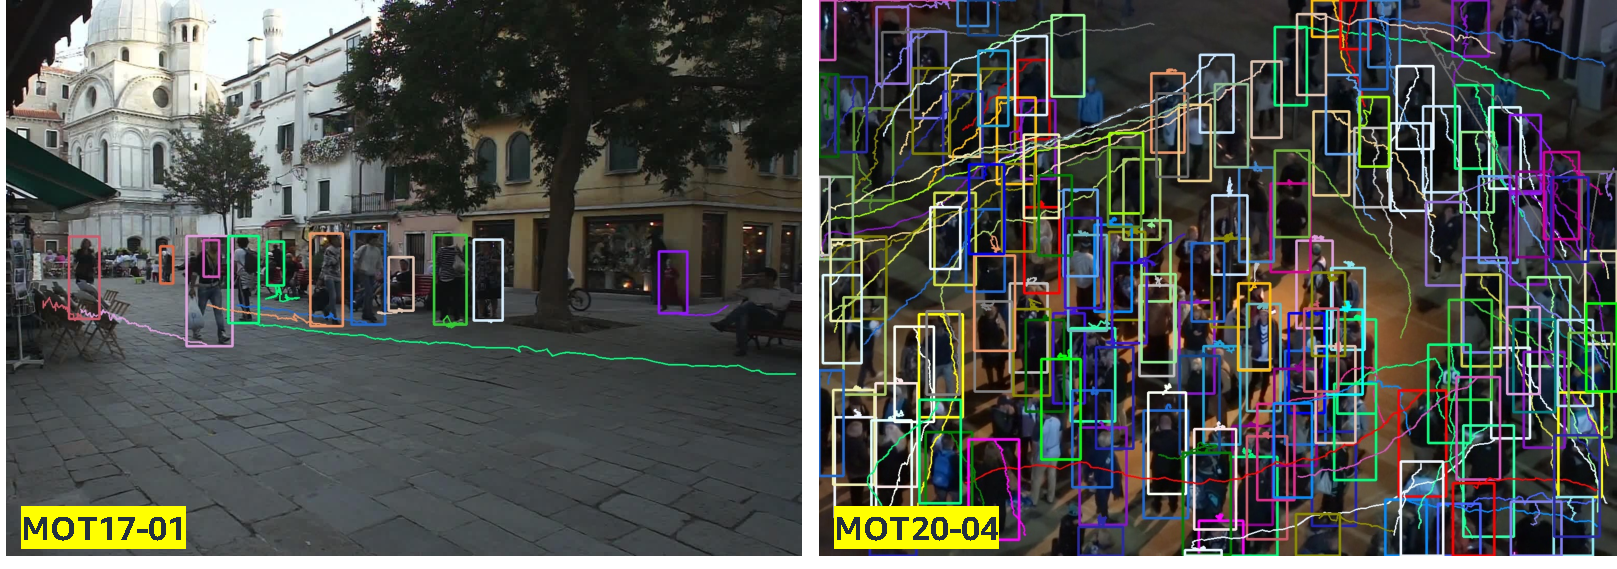
\includegraphics[width=0.99\linewidth]{figures/result3.pdf}
    \vspace{-1.5mm}
    \caption{
        \textbf{Examples of our tracking performance} on MOT17 and MOT20. Each identity is shown in a colored bounding box and trajectory in the past 150 frames are displayed.}
    \label{fig:vis_result}
    \vspace{-3.0mm}
\end{figure}

\vspace{-4pt}
\vspace{3pt} \noindent \textbf{Results on crowded scenarios}.
MOT20 is a more challenging benchmark with crowded scenarios and serious occlusions.
Table~\ref{tab:MOTexp} shows that MeMOT achieves comparable performance with the state-of-the-art JDE method (FairMOT), but gets 63\% reduction in IDsw.
Note that FairMOT is trained with 8$\times$ more training data than ours.
Comparing to other Transformer-based methods, MeMOT outperforms them by 6.7 IDF1 and 5.2 HOTA.
By getting a much lower IDsw, our learnable association solver shows its advantage to deal with the occlusion problem.
We observe that IoU-based association methods (\eg, TransCenter and TransTrack)
fail to handle frequent occlusion, and for the re-identification feature-based methods (\eg, FairMOT), it is hard to obtain high-quality embeddings to measure inter-object similarity due to the small object sizes.

\begin{figure}
\centering
    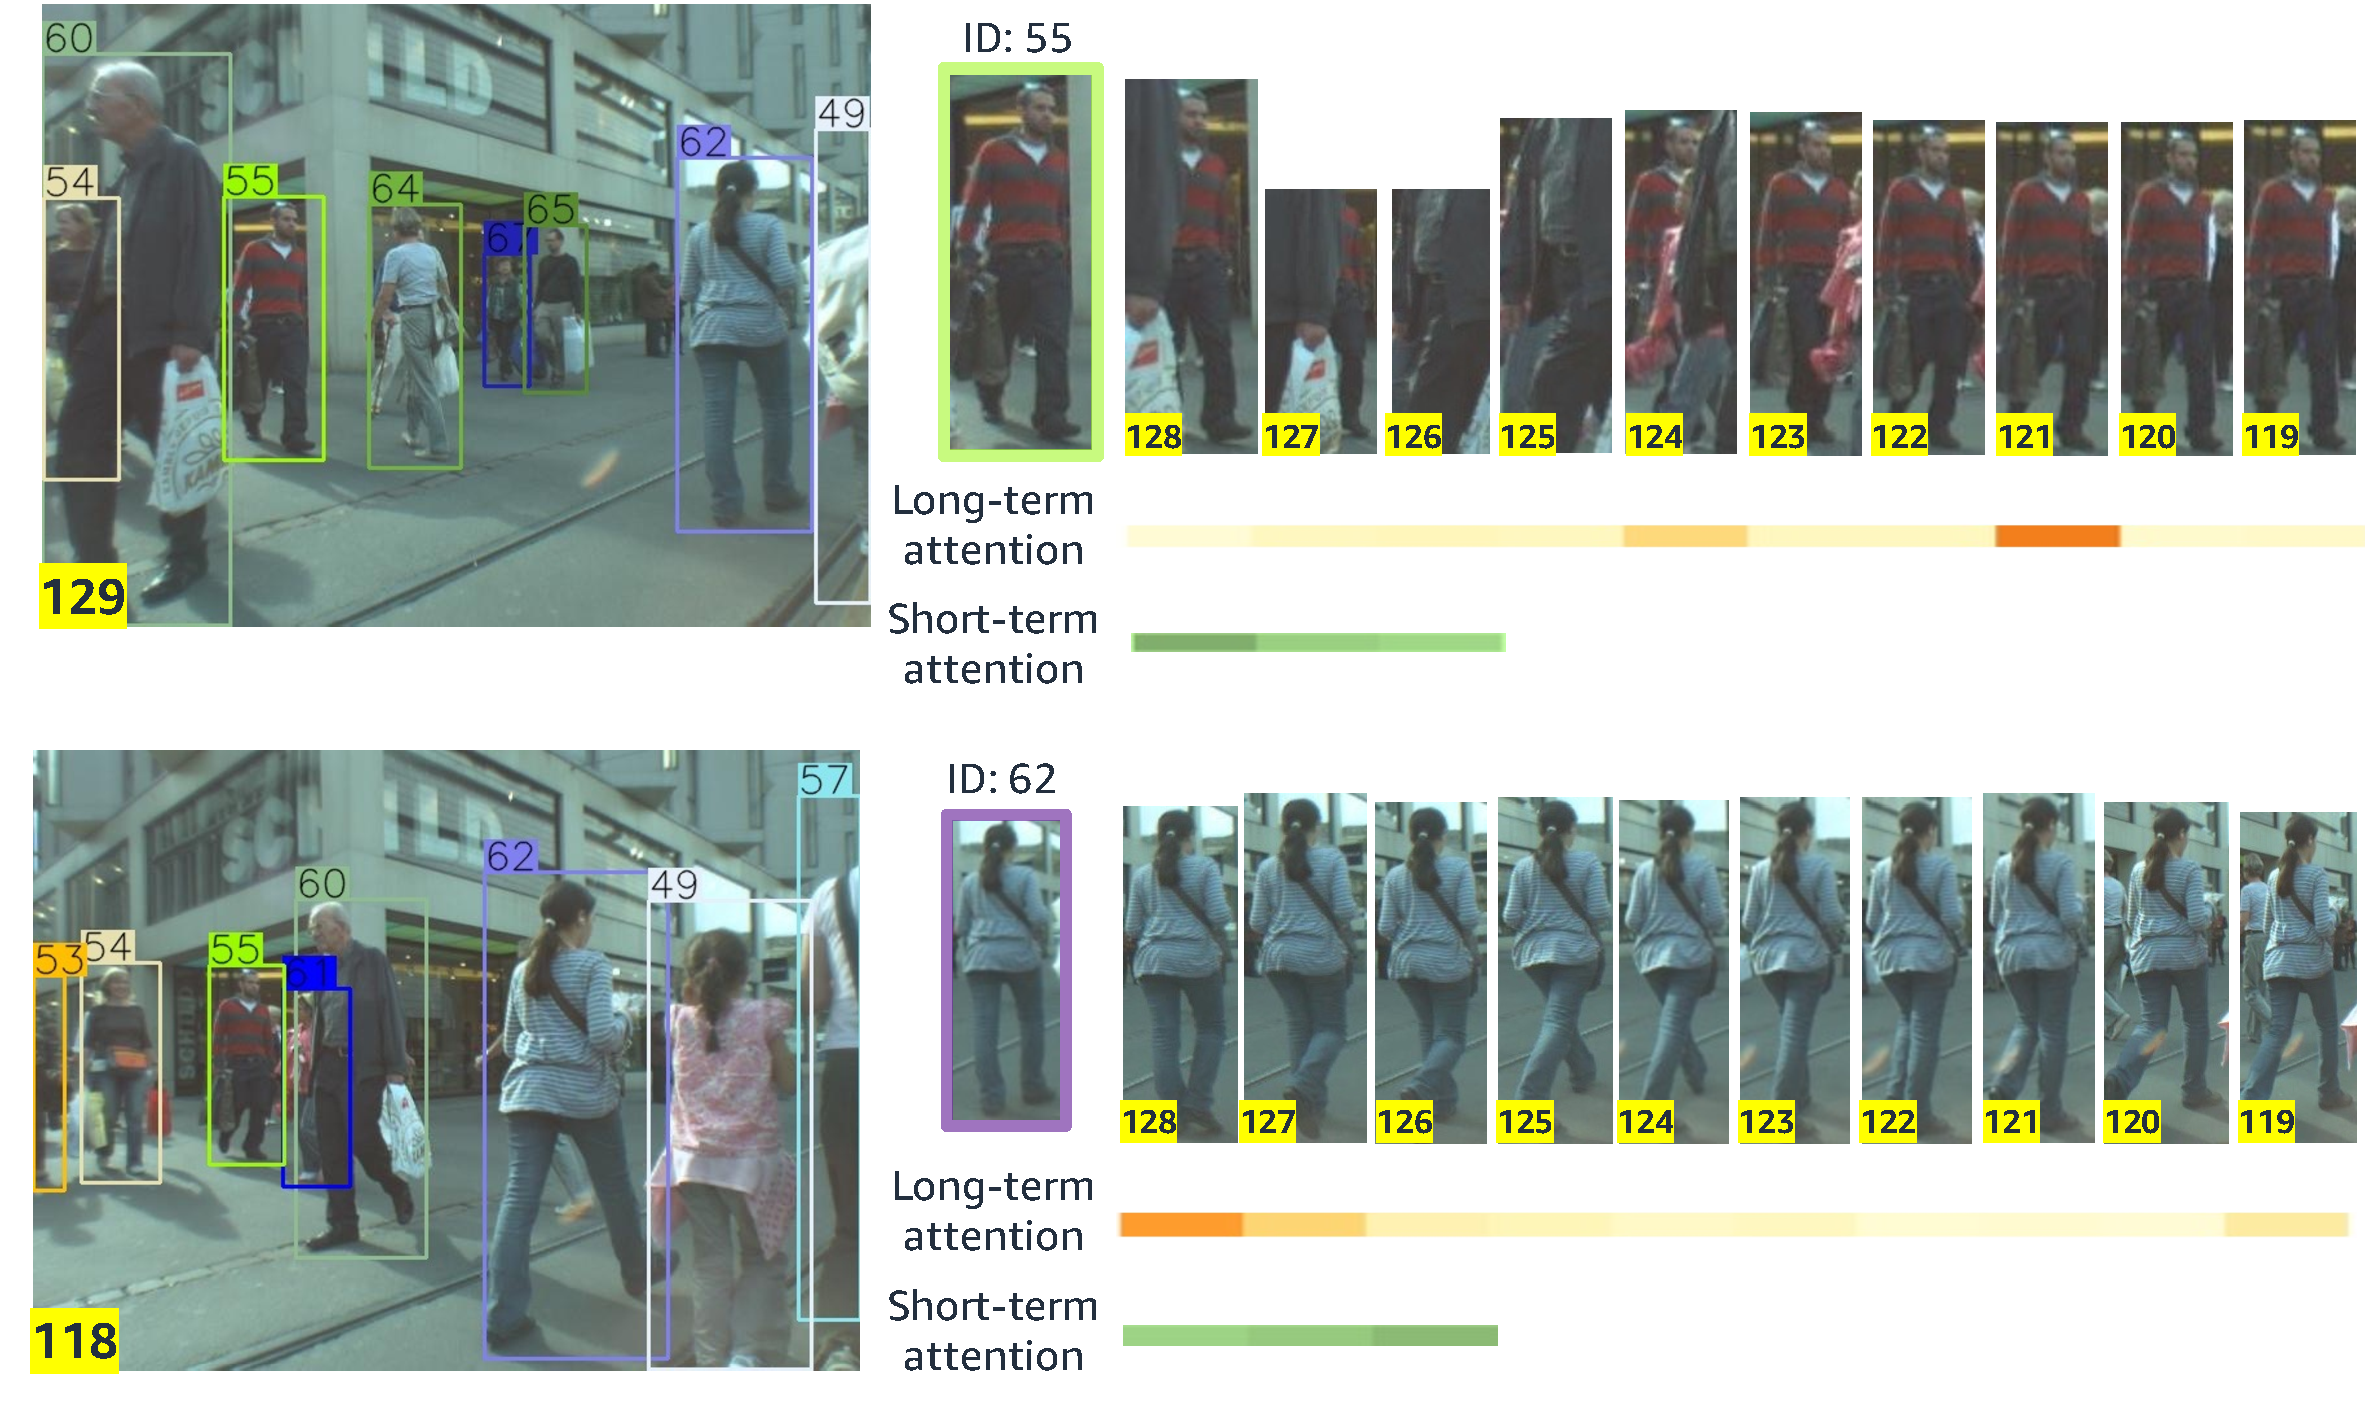
\includegraphics[width=\linewidth]{figures/attention_example.pdf}
    \vspace{-6.0mm}
    \caption{
    \textbf{Visualization of long- and short-term attentions}.
    \textbf{Left}: Tracking results of frame 118 and 129, where tracked objects are displayed in colors with confidence scores.
    \textbf{Right}: Learned long- and short-term attention maps for the intermediate frames of two selected identities (\ie, ID 55 and 62). Darker color represents stronger attention.}
    \label{fig:vis_attn}
    \vspace{-2.5mm}
\end{figure}

\vspace{-1mm}
\subsection{Visualization}
\label{sec:exp:qualitative}
\vspace{-1mm}

Object trajectories are visualized in Fig.~\ref{fig:vis_result}. Results of MOT17-01 show that MeMOT generates long, consistent predictions even when objects pass by each other frequently. Results on MOT20-04 suggest MeMOT's superior object detection and association ability in crowd scenarios. Due to the small object size and poor lighting, feature similarity-based association methods~\cite{zhang2020fair,wang2019towards} are precarious, causing higher IDsw. We provide video demos in the supplementary material for detailed comparison.

In Fig.~\ref{fig:vis_attn}, we also visualize the attention weights of the memory aggregator to elaborate what information is referenced from the memory. For object 55, who is occluded by object 60 from frame 125 to 128, the embedding right before occlusion (frame 124) and a full-body feature (frame 121) contribute the most to re-linking (frame 129) after occlusion. And his short-term attention weights are higher on a less-occluded frame (frame 128) than fully-occluded frames (frame 126 and 127).
As for a non-occluded object (\ie, object 62), attention weights are higher on the short-term memory (frame 126 to 128) and the far-away frames are less attended. These observations validate that our memory aggregator is capable of capturing distinctive object features, especially when objects are crossing each other.

\subsection{Ablation Studies}
\label{sec:exp:ablation}

We experiment with different memory and model design choices.
Unless noted otherwise, we use trimmed models by reducing their number of layers of all Transformer units from 4 to 2.
% The longer side of input frames is reduced to $1333$ pixels.
The models are trained on MOT17 training set and validated on MOT15 training set. Validation videos that are overlapped with the training set are excluded.

\vspace{3pt} \noindent \textbf{Effect of short-term memory length}.
Table~\ref{tab:ablation:memory_length_short} compares the performance using different short-term memory lengths, by keeping the long-term memory length $T_l$ as 24.
It shows that only using the last two observations (\ie, $T_s$=$2$) for short-term memory aggregation slightly decreases the performance.
This observation is consistent with results in prior work~\cite{sun2020transtrack,meinhardt2021trackformer} that propagates tracking results only between adjacent frames.
On the other hand, increasing the short-term length from 3 to 5 does not make a big difference.
We think these information gaps are compensated by the long-term memory.
Considering the accuracy-efficiency trade-off, we set $T_s$ to 3 as default in other experiments.    

\begin{table}
\centering
\footnotesize
\begin{tabular}{cc|cccccc}
\toprule[1.5pt]
        \textbf{$T_s$} & \textbf{$T_l$} & \textbf{IDF1} & \textbf{MOTA} & \textbf{HOTA} & \textbf{IDsw} & \textbf{DetA} & \textbf{AssA} \\\hline
         2 & \multirow{4}{*}{24} & 72.52& 65.62& 58.99& \textbf{76}& 56.97& 62.14\\
        3 & &\textbf{73.15}& \textbf{68.08}& \textbf{59.75} & 93 & \textbf{57.92} & \textbf{63.10}\\
        4 & &72.40 & 67.11& 59.51 & 93& 57.58& 62.82\\
        5 & &72.75 & 66.65 & 59.48& 92& 57.42& 62.87\\
\bottomrule[1.5pt]
    \end{tabular}
\vspace{-2.0mm}
\caption{Comparisons on different length of short-term memory.}
\vspace{-2.0mm}
\label{tab:ablation:memory_length_short}
\end{table}
\begin{table}
\centering
\footnotesize
%\setlength\tabcolsep{5.0pt}
\begin{tabular}{cc|cccccc}
\toprule[1.5pt]
        \textbf{$T_s$} & \textbf{$T_l$} & \textbf{IDF1} & \textbf{MOTA} & \textbf{HOTA} & \textbf{IDsw} & \textbf{DetA} & \textbf{AssA} \\\hline
        \multirow{5}{*}{3} & 3 & 71.27 & 67.14 & 59.09 & 136 &57.85& 61.41\\
        & 5 & 71.70 & 67.94 & 59.31 & 136 & 58.24 & 61.50\\
        & 10 & 71.66 & \textbf{68.29}& 59.53 & 117 & \textbf{58.35} & 59.49\\
        & 20 & 72.83&  68.21 & \textbf{59.85} & 96& 58.03 & 63.00\\
        & 24 & \textbf{73.15}& 68.08& 59.75 & \textbf{93} & 57.92 & \textbf{63.10}\\
\bottomrule[1.5pt]
    \end{tabular}
\vspace{-2.0mm}
\caption{Comparisons on different length of long-term memory.}
\label{tab:ablation:memory_length_long}
\vspace{-2.0mm}
\end{table}
\begin{table}
\centering
\footnotesize
%\setlength\tabcolsep{5.0pt}
\begin{tabular}{cc|cccccc}
\toprule[1.5pt]
        \textbf{$q_s$}  & \textbf{$q_l$} & \textbf{IDF1} & \textbf{MOTA} & \textbf{HOTA} & \textbf{IDsw} & \textbf{DetA} & \textbf{AssA} \\\hline
        & \checkmark  & \textbf{73.15}& 68.08 & \textbf{59.75}& \textbf{93}& 57.92 & 63.10\\
        \checkmark  & & 67.25 & \textbf{69.88} & 57.36 & 112 & \textbf{58.01} & 61.76\\
        \checkmark  & \checkmark & 41.09& 59.80& 43.28& 207 & 45.36 & 38.52\\
        & & 72.30 & 62.68 & 58.84 & 103 & 55.72 & \textbf{63.37}\\
\bottomrule[1.5pt]
    \end{tabular}
    \vspace{-2.0mm}
\caption{Comparisons on different configuration of the short-term cross-attention query $q_s$ and long-term cross-attention query $q_l$.}
%\caption{Comparisons on different configuration of the short-term cross-attention query $q_s$ and long-term cross-attention query $q_l$. Empty means using the latest observation, $\checkmark$ represents the query is learnable and recursively updated during inference. Our MeMoT design (row-1) yields best overall performance. }
\label{tab:ablation:learn}
\vspace{-2.0mm}
\end{table}

\vspace{3pt} \noindent \textbf{Effect of long-term memory length}.
MeMOT uses a long-term memory to mitigate the occlusion problem.
Table~\ref{tab:ablation:memory_length_long} shows the effect of different long-term memory lengths $T_l$ from 3 to 24.
Note that we set the max length as 24 due to hardware limitation.
As $T_l$ grows, the association performance keeps increasing with fewer IDsw and higher IDF1.

\vspace{3pt} \noindent \textbf{Comparing to heuristic memory aggregations}.
We explore the design of memory aggregation module by first comparing to heuristic algorithms.
Considering the tracklet length can be relatively long (up to 24),
we do not concatenate the embeddings but test the pooling methods.
Then the aggregation can be conducted by using either arithmetic mean or maximum norm over the most recent $T$ frames.
Table~\ref{tab:ablation:mem_structure_heuristic} shows that using these simple pooling methods is incapable of capturing informative track features, resulting in a huge performance drop in IDF1 and MOTA.

\vspace{3pt} \noindent \textbf{Comparing to attention-based memory aggregations}.
We experiment with another two attention-based aggregation designs in memory encoding.
The first one is to only use a cross-attention module, without the separation of long and short memory.
This baseline uses the latest observation to query an object's past $T$ embeddings.
As shown in Table~\ref{tab:ablation:mem_structure_attn}, it produces worse association performance, with -0.51\% and -0.34\% MOTA for $T=3$ and $T=24$, respectively.
The IDsw also increases by 6 and 44.
Inspired by LSTR~\cite{xu2021long}, the second one is to use the aggregated short-term embeddings to retrieve useful information from the long-term memory. The result shows that this design also decreases the performance. We argue that, in the action detection task that LSTR focuses on, the result of each frame is independent and deficient short-term features have a limited effect on future predictions. However, association errors can propagate in MOT, thus using long-term features to compensate for short-term features is more desirable. 

\begin{table}
\centering
\footnotesize
%\setlength\tabcolsep{5.0pt}
\begin{tabular}{c|c|cccc}
\toprule[1.5pt]
        \textbf{Method} & \textbf{Parameter} &\textbf{IDF1} & \textbf{MOTA} & \textbf{HOTA} & \textbf{IDs} \\\hline
        Ours & - &\textbf{73.15}& \textbf{68.08}& \textbf{59.75}& \textbf{93}\\\hline
        \multirow{4}{*}{Pooling}& Average (T=3) & 25.04& 30.72 & 21.89 & 267\\
        & Max (T=3) & 46.83& 41.28& 35.44& 235\\ 
        & Average (T=24) & -& -7.29& -& -\\
        & Max (T=24) & 25.78& 10.20& 6.54& 332\\
\bottomrule[1.5pt]
    \end{tabular}
    \vspace{-2.0mm}
\caption{Comparisons with heuristic memory aggregation design.}
%\caption{Comparisons with heuristic memory aggregation design. The result shows simple heuristic aggregation methods are incapable of extracting instance features for tracking, even given the long-term memory. Our proposed memory aggregator yields significantly better tracking performance.}
\label{tab:ablation:mem_structure_heuristic}
\vspace{-2.0mm}
\end{table}
\begin{table}
\footnotesize
%\setlength\tabcolsep{5.0pt}
\begin{tabular}{c|c|cccc}
\toprule[1.5pt]
        \textbf{Method} & \textbf{Parameter} &\textbf{IDF1} & \textbf{MOTA} & \textbf{HOTA} & \textbf{IDs} \\\hline
        Ours & - &\textbf{73.15}& 68.08& \textbf{59.75}& \textbf{93}\\\hline
        \multirow{2}{*}{Single}& T=3 & 72.64 & \textbf{68.74} & 58.94 & 137\\
        & T=24 & 72.81 & 66.25 & 58.73 & 99\\\hline
        \makecell{Long-after-short} & - & 70.30 & 65.39& 57.03 & 101\\
\bottomrule[1.5pt]
\end{tabular}
\vspace{-2.0mm}
\caption{Comparisons on adaptive memory aggregation design.}
\label{tab:ablation:mem_structure_attn}
\vspace{-2.0mm}
\end{table}
\begin{table}[t]
\centering
\footnotesize
%\setlength\tabcolsep{5.0pt}
\begin{tabular}{c|cccccc}
\toprule[1.5pt]
        \textbf{Update}  & \textbf{IDF1} & \textbf{MOTA} & \textbf{HOTA} & \textbf{IDsw} & \textbf{DetA} & \textbf{AssA} \\\hline
        \checkmark  & \textbf{73.15}& \textbf{68.08}& \textbf{59.75} & \textbf{93} & \textbf{57.92} & \textbf{63.10}\\
         & 61.03 & 43.42 & 49.24 & 161 & 42.40 & 57.96 \\
\bottomrule[1.5pt]
    \end{tabular}
    \vspace{-2.0mm}
\caption{Comparison on the updating of $\mathbi{Q}_{dmat}$.}
\label{tab:ablation:update}
\vspace{-2.0mm}
\end{table}
\begin{table}
\footnotesize
%\setlength\tabcolsep{5.0pt}
\begin{tabular}{c|cccccc}
\toprule[1.5pt]
        \textbf{Confidence} & \textbf{IDF1} & \textbf{MOTA} & \textbf{HOTA} & \textbf{IDs}& \textbf{DetA} & \textbf{AssA} \\\hline
        Single& 69.09& 63.51& 52.86& 104& 55.76 & 61.77\\
        Dual & \textbf{73.15}& \textbf{68.08}& \textbf{59.75} & \textbf{93} & \textbf{57.92} & \textbf{63.10}\\
\bottomrule[1.5pt]
    \end{tabular}
\vspace{-2.0mm}
\caption{Comparisons between single and dual confident scores.}
\label{tab:ablation:novelty}
\vspace{-2.0mm}
\end{table}

\vspace{3pt} \noindent \textbf{Using learnable tokens vs. latest observation for memory aggregation}.
We explore using either the learnable tokens or the latest observation for long- and short-term memory aggregation, as shown in Table~\ref{tab:ablation:learn}.
For the short-term token (row2 vs. row4), using the latest observation (row4) yields better association performance (+5.05 IDF1).
After fixing the short-term token, using learnable tokens for long-term memory aggregation obtains slightly better performance (row1 vs. row4), with +0.85 IDF1 and -10 IDsw.
It is worth noting that using learnable tokens for both long- and short-term branches is risky, getting the IDF1 and MOTA drop to 41.09\% and 59.80\%.
These observations validate our intuition for separating the long- and short-term branches.
1) Due to the temporal variance, the long-term memory may be less informative to match the latest observation but provides diverse features within a tracklet.
To extract the supportive context information, using learnable tokens is more effective.
2) Short-term memory features share a high similarity, thus directly querying them with the latest observation can smooth out the noises.
3) These two branches can acquire complementary information.

\vspace{3pt} \noindent \textbf{Dynamic update of memory aggregation tokens}.
Since we model online tracking as an iterative process, it is worth studying if the long-term memory aggregation tokens should be updated during inference.
Results in Table~\ref{tab:ablation:update} shows that dynamically updating the queries with the most recent information contributes to better detection and tracking performance. By passing the firsthand observation to the long-term queries, more detailed information for current association is extracted, rather than general information.

\vspace{3pt} \noindent \textbf{Effect of uniqueness score for training MeMOT}.
We introduce the uniqueness score to link new detections with the tracked objects and reject false positives.
Here we evaluate its contribution by removing the prediction branch of uniqueness score, as shown in Table~\ref{tab:ablation:novelty}.
Without the uniqueness branch (single output), there are more false positive detections and IDsw.
We separate the mixed meanings of the output classification score by splitting the prediction of objectness and uniqueness into two heads. In a single-head architecture, for tracked object queries, the score means the confidence of existence; for the proposal queries, it means the confidence of being a new-born object. While the two purposes share the same classification layer, low confidence values are ambiguous: it means non-objectness, or not a new object. Our design removes the ambiguity and avoids under-training of the classification layers.

\subsection{Limitations}
\label{sec:exp:limitations}

As MeMOT is currently trained with supervised learning, it requires video datasets with tracking annotation. 
However, existing datasets for tracking are still limited in size and diversities, due to the high cost of annotating videos. 
Developing annotation efficient training methods is crucial to overcoming this difficulty.
Although the spatio-temporal memory is shown to be effective in tracking objects consistently, it indeed increases the GPU memory cost in training. This limits the temporal length of the memory and therefore calls for further improvement in efficiency.
